\section{Implementation}
An architecture is proposed for Trend Analysis and Issue Tracking. Each problem is solved by combining modules and output of Trend Analysis could be processed to be the input of Issue Tracking task. Some analyses are also conducted to find the most suitable and sufficient solution for each part of solution.
The architecture is depicted as following.
\begin{figure}[h]
\centering
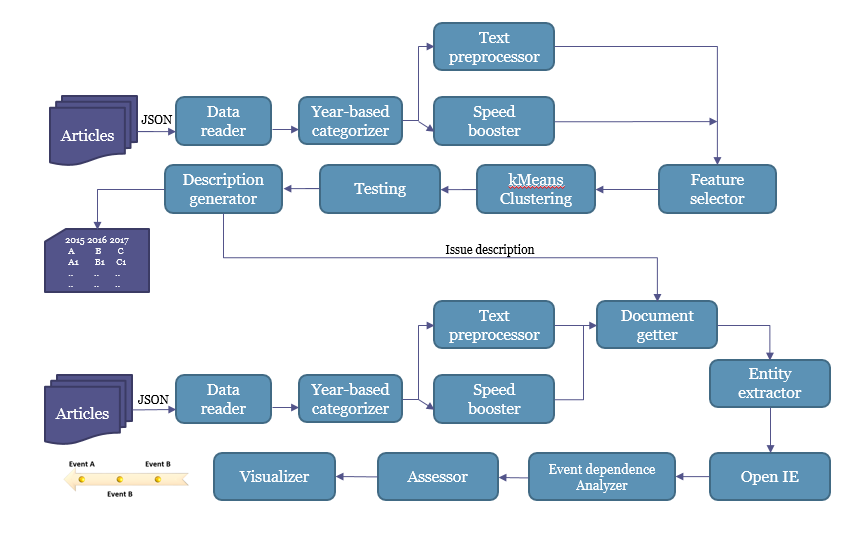
\includegraphics[scale= 0.4]{work_flow.png}
\caption{Workflow of Trend Analysis and Issue Tracking}
\end{figure}
The model extracts the top trends of 3 years and detects relations among the events as much as possible.
\subsection{Trend Analysis}
\subsubsection{Data Reader}
The given corpus is in JSON format, then we use JSON module in Python to read the input data files. As we have several section for an article, dataframe in pandas module is the most sufficient data structure to store dataset. 
From dataframe, sorting articles by times ascendingly help further steps.
\subsubsection{Year-based Categorizer}
There are 4 years of article publishments are 2015, 2016, 2017 and 2018. However, 2018’s articles are aggregated to 2017 group as the publish date is the first date of 2018. From that point, we counted the numbers of documents 
for years and separate based on the ascendingly-ordered time article dataframe from data reader. 
\begin{figure}[h]
\centering
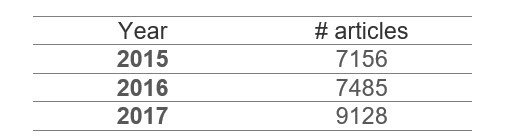
\includegraphics[scale= 0.6]{table_1.png}
\caption{Numbers of articles per year}
\end{figure}
\subsubsection{Speed Booster}
Although a progress bar is constructed along side with processing, the program takes long time in our PC (Intel core i7-6700, 16GB of RAM and 1TB of HDD): about 10 minutes for each year.

\begin{figure}[h]
\centering
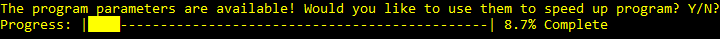
\includegraphics[scale= 0.4]{fig1.png}
\caption{Working of Speed Booster}
\end{figure}

As we analyzed, most of processing time is dedicated for preprocessing while NTLK has to process token-by-token, so we group unchanged parameters and dumped the data using pickle modules. At least, output of preprocessing and even Named Entity Recognition and Ollie could be done in this way to reduce execution time dramatically. Each time running the program, the program detect existence of pickle files and ask users to use available parameters to boost up the speed. Ignoring this if dataset changed to you want to run the program from the beginning to validate it.
\subsubsection{Text Preprocessor}
Since we have raw text as input, we need to preprocess data. This stage consists of some tasks:
\begin{description}
\item[--]Normalization: Convert all text to lower case or upper case to ensure consistency of input. For this task, converting all the words in collection into lower case.
\item[--]Tokenization: Chop documents to pieces and throwing away some certain character such as punctuation, white space, using NLTK tokenizer to get tokens from collection.
\item[-- ]Stemming: This technique are popular in preprocessing, but its two sides of the coin, frequently getting meaningless word like “hi”, “ha”, “wa”, then ignoring this technique because trend analysis require fine-grained output from processing.
\item[--] Lemmatization: Group together the different inflected forms of a word so they can be analyzed as a single item. The NLTK Lemmatization method is based on WordNet’s built-in morph function.
\end{description}
Each article give a set of tokens, relatively much, then we built vocabulary which is the combination of these token sets, and using stop words to filter insignificant words. With each preprocessing technique is added or removed, the number of entries in vocabulary can be changed slightly with the same input dataset.
\subsubsection{Feature Selection}
To speed up the clustering, we wanted to reduce the dimensionality of our model by using feature selection. As Sklearn provides an implementation for feature selection by a variance threshold as well as an option to filter by document frequency, we tried out both of these options.
However for both implementations we found that it was very difficult to control the amount of features to be selected.

We decided to use document frequency as it was faster and more easy to use.

\begin{figure}[h]
\centering
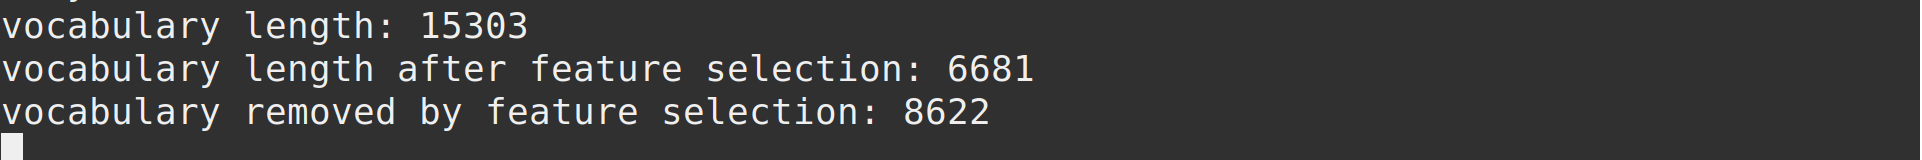
\includegraphics[scale= 0.15]{feature_selection.png}
\caption{Vocabulary size by feature selection}
\end{figure}

\subsubsection{Clustering}
For clustering the features extracted before, we used the k-means++ implementation of Sklearn. Our resulting parameters for the clustering are 100 iterations, 10 consecutive runs and k equals 149. The 10 consecutive runs define the number of runs the k-means++ runs with different cluster centroid seeds and the best one in terms of the sum of squared distances of each article to their cluster center is the cluster result. However we did not start with k equals 149 at the first place, in order to find this k value we had to run the algorithm several times with different values for k. The k values we tried were between 100 and 200 and we evaluated the best k whilst writing the article headings of our top ten clusters to a file. In addition we wrote the sum of squared distances of the articles to their cluster center to the same file. After, we had a look at the text file and decided if it was a good result or not. However, because we start with random initial cluster centroids, we have a slightly different result with every execution. Further, we decided that our top ten clusters are not the ten clusters with the most articles because with k values between 100 and 200 we end up with some clusters that have more than 400 articles. And for those it was really hard to find a description. Because of that we choose the ten clusters with the most articles but less than 150 articles which gave us a good result and well defined top ten clusters.

\subsubsection{Description creation}
The descriptions for the top ten issues of each year is done manually by reading the headings of the articles of the top ten clusters and writing a suitable description for them. Our first idea was to use the features of the cluster and use them to automatically write a description, however that was too hard and that is why we ended up doing it manually by hand.

\subsection{Issue Tracking}

\subsubsection{Getting Documents}
As we didn't want to rely on the clustering result of the previous task, we used Cosine Similarity to obtain articles related to an issue.
As Gensim provides an implementation of Cosine Similarity as well of LSI (Latent Semantic Indexing), which transforms the documents into a latent space of a lower dimensionality \parencite{gensim}.
We wrote a description for each article which is read by our program and use Cosine Similarity to retrieve a user-specified number of documents that are most similar to the description. This list of articles is then used for further analysis.
=======
Gensim provides an implementation of Cosine Similarity as well of LSI (Latent Semantic Indexing), which transforms the documents into a latent space of a lower dimensionality \parencite{gensim}.
We wrote a description for each article which is read by our program and use Cosine Similarity to retrieve a user-specified number of documents that are most similar to the description. This list of articles is then used for further analysis.
\begin{figure}[h]
\centering
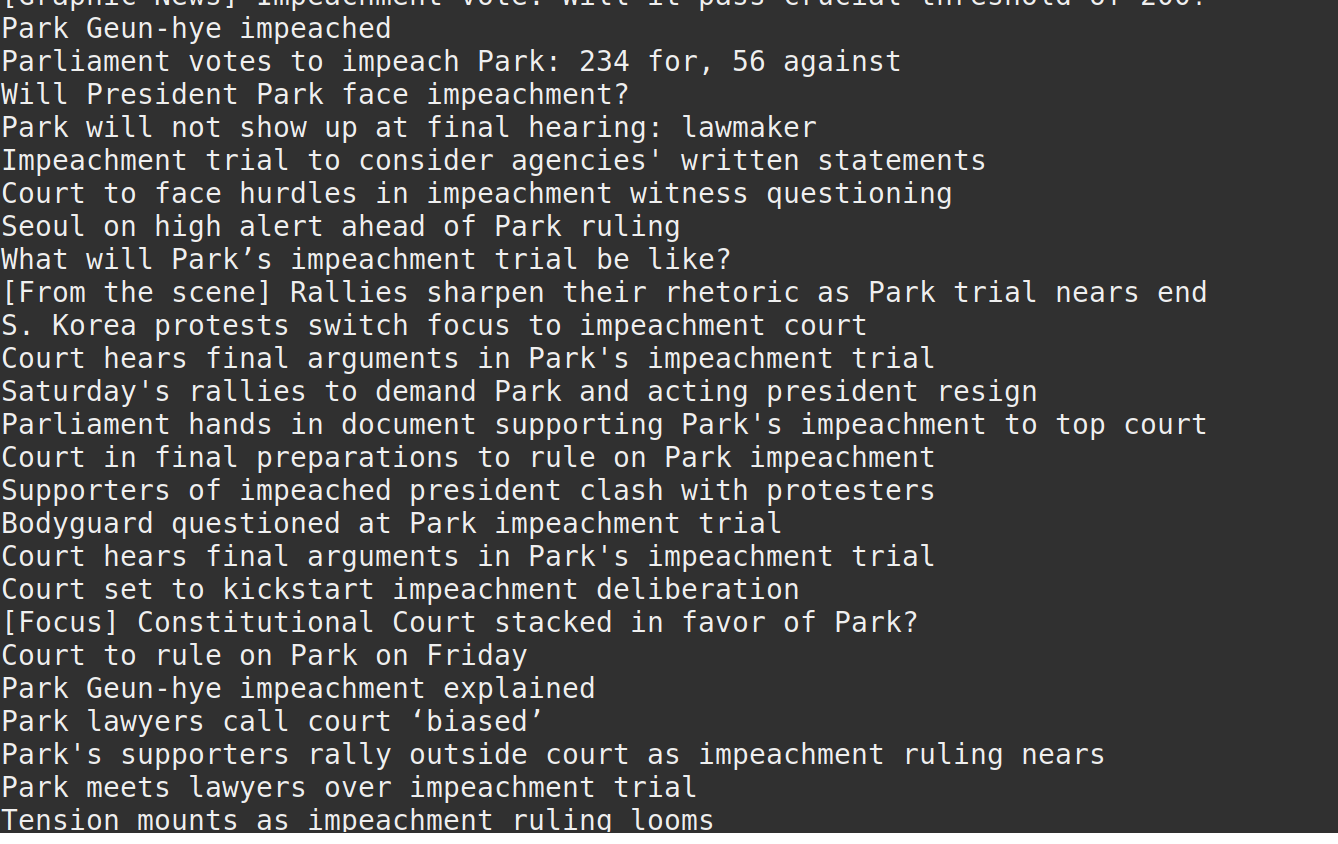
\includegraphics[scale= 0.2]{similarity.png}
\caption{Result of Similarity Query (Article Headings related to the Impeachment of President Park)}
\end{figure}

\subsubsection{Named Entity Recognition}
For each article in corpus, extracting entities such as person name, location, time, organization gives more accurate knowledge about events in the article. Few state-of-the-art tools were taken into consideration, but there are three most famous libraries: Spacy, NLTK and CoreNLP. Below table compares Spacy with CoreNLP and NLTK in NER task.
\begin{figure}[h]
\centering
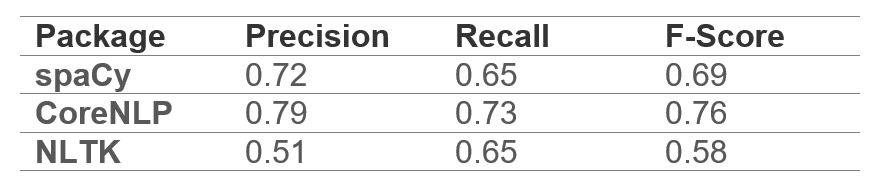
\includegraphics[scale= 0.35]{table_2.png}
\caption{Performance comparison of NLP tools \parencite{analytics_vidhya_misc}}
\end{figure}
Spacy and CoreNLP are significantly better than NLTK in this task in term of performance. However, CoreNLP does not provide Python API, and the performance gap between Spacy and CoreNLP is tolerant. Thus, we sacrificed accuracy to obtain ease and consistency in implementation. The speed of Spacy, although not the most important factor in our work, could also be an advantage of Spacy over CoreNLP.
\begin{figure}[h]
\centering
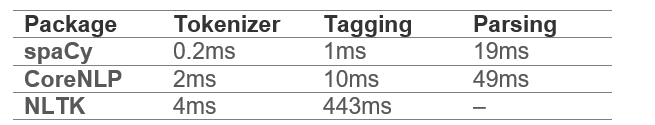
\includegraphics[scale= 0.5]{table_3.png}
\caption{Execution time comparison of NLP tools \parencite{analytics_vidhya_misc}}
\end{figure}
Spacy returns pairs:\textit{\textbf{ (entity , entityType)}}, so a large number of types entity types, but we just captured 5 types:
\begin{figure}[h]
\centering
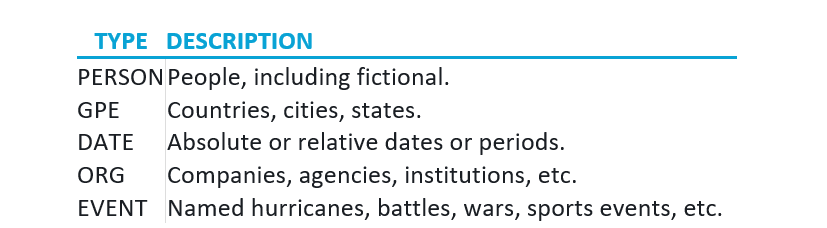
\includegraphics[scale= 0.5]{table_4.png}
\caption{Expected entity types \parencite{spacy_ling_misc}}
\end{figure}
Recognition errors are sometimes attributable to Spacy as it detects “Yophap” or “Zika” as person name, “Park” as location, “H5N1” as organization. Unformatted text as input also results in wrong entities. To increase accuracy in NER, rules are added to filter to put entities to their correct places, but this kind of manual work is effort-consuming and domain-specific when we need to look at the result to see the most frequently-committed mistakes and correct them. Spacy still has a long way to go.
\subsubsection{Relation Extraction}
\textbf{OLLIE for Relation Extraction}\\
Among techniques todays for Information Extraction, we chose Open Information Extraction for its advantages over others.  Hand-labeled data (documents on a specificName topic) and pre-specified relations (supervised learning) are required in traditional IE systems. However, such kind of system is limited because of their supervised natured, then not able to scale to word wide web \parencite{sinamiran_misc}. 
\begin{figure}[h]
\centering
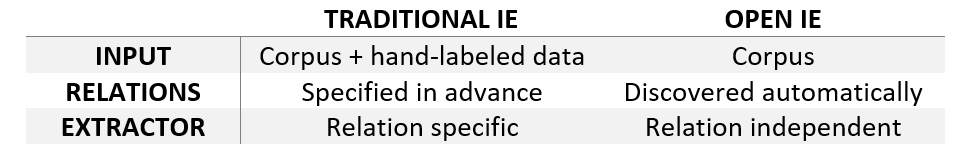
\includegraphics[scale= 0.3]{table_5.png}
\caption{Comparison between Traditional and Open IE}
\end{figure}
With the given dataset, Open-IE is selected for its merits:
\begin{description}
\item[--]Avoid hand-labeling data.
\item[--]Single pass over corpus.
\item[--]No pre-specified vocabulary.
\end{description}
Open Information Extraction (IE) systems extract relational tuples from text, without requiring a pre-specified vocabulary, by identifying relation phrases and associated arguments in arbitrary sentences. However, state-of-the-art Open IE systems, ReVerb (Fader et al., 2011; Etzioni et al., 2011) and WOE\textsuperscript{\textit{parse}} (Wu and Weld, 2010) share two important weaknesses \parencite{schmitz2012open} that degrade the performance of Open IE.
\begin{description}
\item[--]Expanding the syntactic scope of relation phrases to cover a much larger number of expressions.
\item[--]Expanding the Open IE representation to allow additional context information such as attribution and clausal modifiers.
\end{description}
OLLIE extractions obtain a considerably higher yield at higher or comparable precision relative to existing systems while ReVerb seems to be suitable with small dataset, and WOE\textsuperscript{\textit{parse}} to have lower precision and yield.
\begin{figure}[h]
\centering
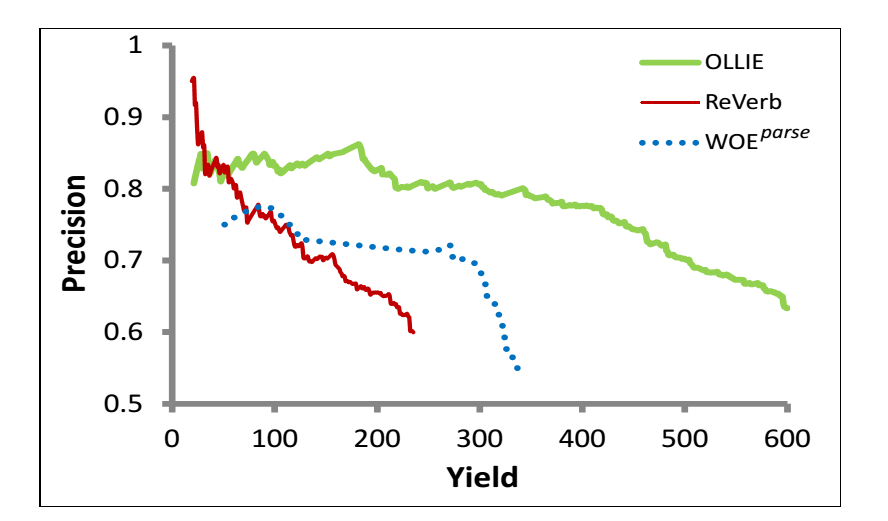
\includegraphics[scale= 0.35]{openie_comparison.png}
\caption{Comparison of different Open IE systems \parencite{schmitz2012open}}
\end{figure}
\textbf{OLLIE post-processing}\\
OLLIE expands and covers much larger of number of relation expressions, thus causing duplicated tuples. Tuples are defined as:
$$t = (e_i, r_{i,j}, e_j)$$
Where $e_i, e_j$ are entities (strings) and $r_{i,j}$ is the relation between them (string).
% \begin{figure}[h]
% \centering
% 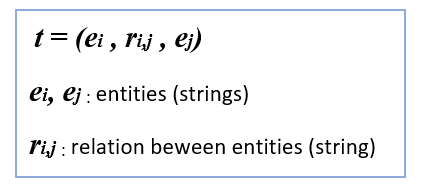
\includegraphics[scale= 0.5]{equation_1.png}
% \end{figure}
Furthermore, OLLIE introduces enabling condition which is a condition that needs to be met for the extraction to be true. Certain words demark an enabling condition, such as "if" and "when". Ollie captures enabling conditions if they are present.
\begin{figure}[h]
\centering
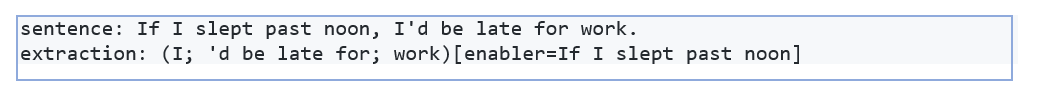
\includegraphics[scale= 0.35]{txt_1.png}
\caption{TODO}
\end{figure}
As we analyzed in the output of OLLIE, enabler could help identify relations amongst incident.
\begin{figure}[h]
\centering
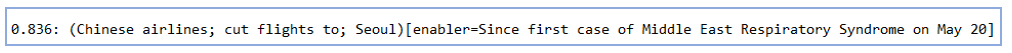
\includegraphics[scale= 0.35]{txt_2.png}
\caption{TODO}
\end{figure}
And as the consequence of expanding expression, OLLIE gives redundancy.
\begin{figure}[h]
\centering
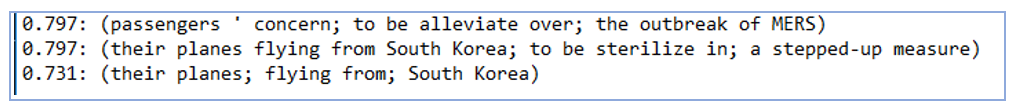
\includegraphics[scale= 0.35]{txt_3.png}
\caption{TODO}
\end{figure}
To remove redundant tuples for an expression, we used \textit{SequenceMatcher} inspired by Ratcliff/Obershelp algorithm to calculate similarity ratio of two strings and discarding with keep the highest confidence score tuples given by OLLIE.
$$D_{ro} = \frac{2\cdot K_m}{|S_1| + |S_2|}$$
Here, \textbf{\textit{K}\textsubscript{\textit{m}}} is a number of \textbf{matching} characters,|S\textsubscript{1}| and |S\textsubscript{2}| are lengths of strings S\textsubscript{1} and S\textsubscript{2} and respectively, \textbf{{\textit{D}\textsubscript{\textit{ro}}}} is the distance calculated by the algorithm.\\
Single pass corpus extractor only generates tuples per sentence, then it is necessary to know which article tuples belong to. Then, we built an \textit{Index Tagger} and \textit{Index Extractor} to get the article index corresponding to tuples. The idea is simple as at the input of OLLIE, a token containing article index (tagger) is attached in article string, and at the output of OLLIE, parsing based on this known token to know article index of tuples (extractor).

\subsubsection{Analyzing Dependent Events}
As we obtained the triples from OLLIE, we wanted to use the information about entity relations to track dependent events. Therefore we chose only to detect follow-up-events that are mentioned in previous articles in a certain form. We chose to filter the following relations and their derivations from triples to predict a follow-up event:
$$r_{dep} = \{plan, call, urge, allow\}$$
This approach assumes a sentence structure as the following examples that we took from the newspaper collection:
\begin{enumerate}
	\item \enquote{North Korea urged South Korea to shift its inter-Korean policy.}
	\item \enquote{The South plans to allow civilian inter-Korean exchanges.}
	\item \enquote{The prosecutors [...] plan for a face-to-face investigation with Park.}
	\item \enquote{The Constitutional Court plans to deliver its final ruling on President Park Geun-hye 's impeachment on Friday.}
\end{enumerate}
As we filtered the triples that contain the above relations, we formed a search query $q$ concatenating the entities for the triples such that $r_{i,j} \in r_{dep}$ holds:
$$q = e_i e_j$$
The search query is supposed to contain information about the person or institution and an action as for example the cases above:
\begin{enumerate}
	\item North Korea South Korea to shift its inter-korean policy
	\item The South civilian inter-Korean exchanges
	\item The court face-to-face investigation with Park
	\item The Constitutional Court deliver its final ruling on President Park Geun-hye 's impeachment on Friday
\end{enumerate}
We used the search query to find the article that is most similar to the search query using Cosine Similarity. The procedure to find the most similar articles was already described above. The result of the search queries above is the following (keeping the same order as above):
\begin{enumerate}
	\item S. Korea calls for peace, reconciliation on inter-Korean summit anniversary
	\item Taekwondo event may spark ‘sports diplomacy’ with NK
	\item Park's lawyers ask Constitutional Court to exclude key evidence
	\item Park's lawyer says to accept impeachment ruling
\end{enumerate}
This approach assumes that the action was planned was actually going to happen and reported in another newspaper article as it is the case for the given examples. If the action didn't happen, the algorithm will only retrieve the article that is most similar to the search query which is not neccessaryly a follow-up event.

\subsubsection{Visualization}
We used the plotly library to visualize the result. The data points represent events distributed over the time on the x-axis. Dependent events are connected with an edge.
\begin{figure}[h]
\centering
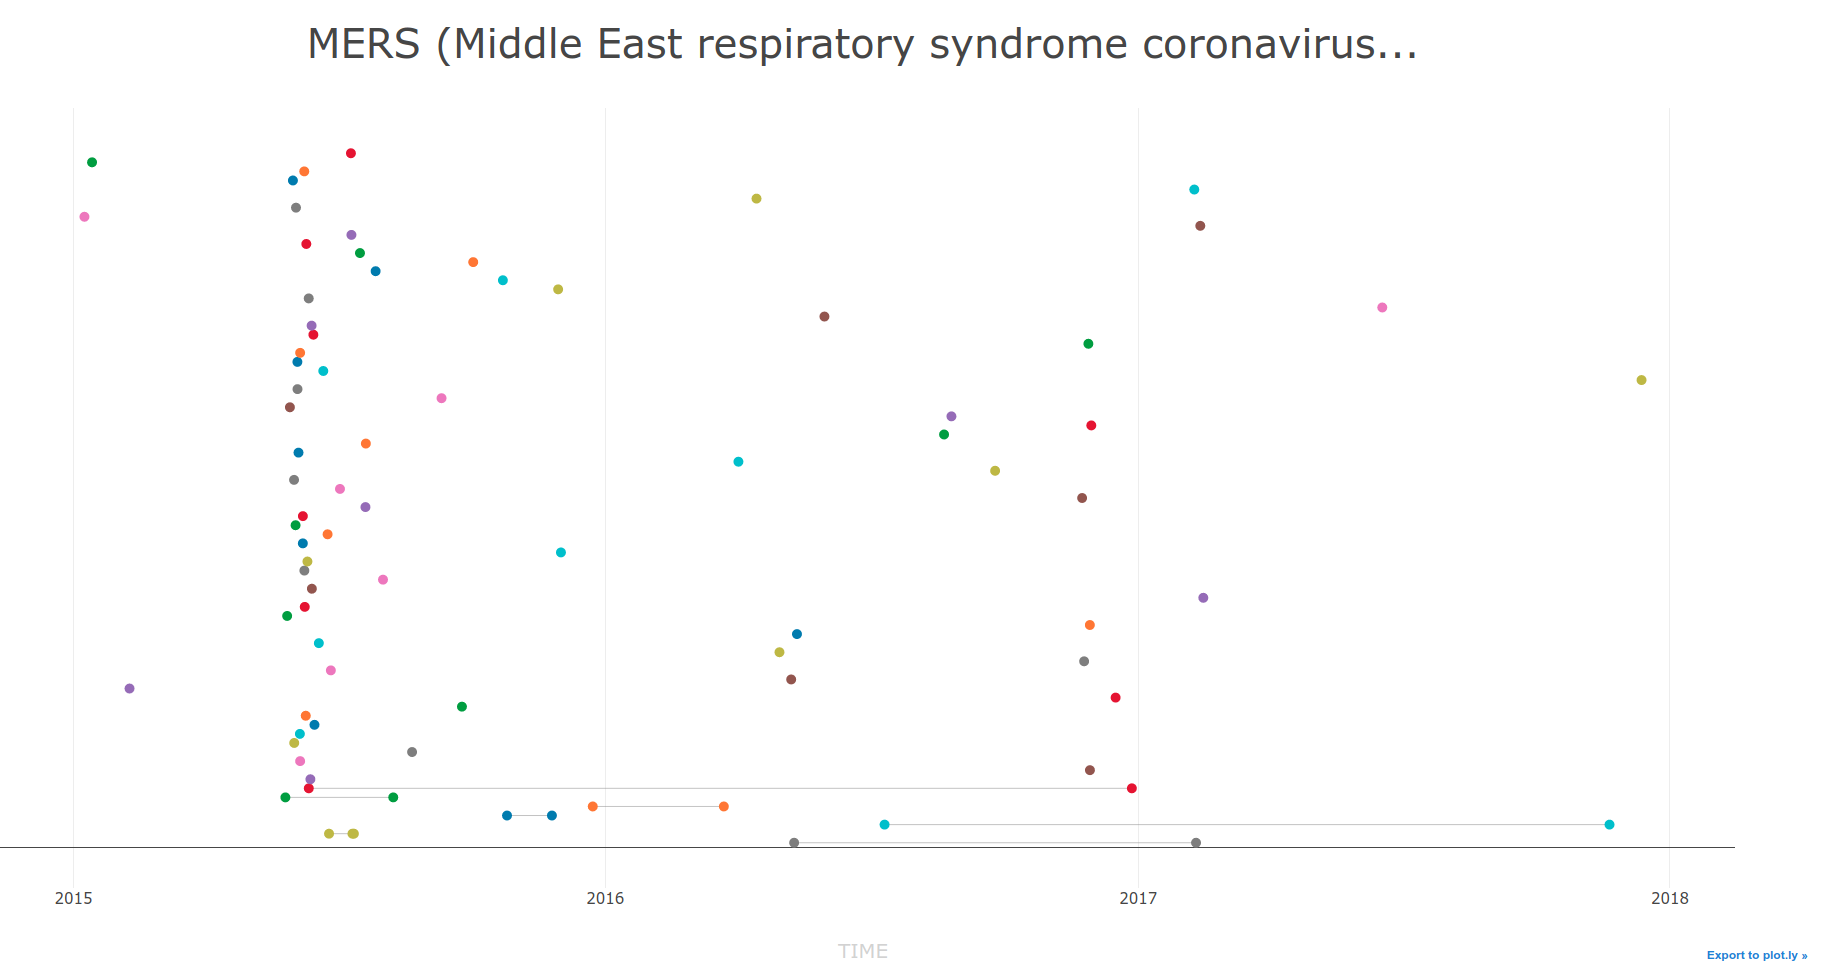
\includegraphics[scale= 0.2]{visualization.png}
\caption{Visualization of MERS Issue Tracking}
\end{figure}

By hovering over the data points the plot also shows the event data.